\subsection{\emph{ROS 2 Node}}
\label{subsec:ros2node}

\emph{ROS 2 node} merupakan komponen utama dari \emph{graph architecture} yang ada pada ROS 2.
\emph{ROS 2 node} umumnya digunakan untuk merepresentasikan suatu proses tunggal yang ada pada robot,
  seperti untuk mengakses motor, mengolah gambar, dan sebagainya \citep{url:understandingros2nodes}.
Setiap \emph{node} yang ada, nantinya dapat berkomunikasi dengan node lain melalui dua cara,
  seperti yang terlihat pada Gambar \ref{fig:diagramnoderos2},
  sebuah \emph{node} dengan \emph{publisher} dapat mengirimkan sebuah data melalui \emph{topic} yang nantinya akan disalurkan ke \emph{node} lain dengan \emph{subscriber} yang terhubung dengan \emph{topic} tersebut.
Selain itu, sebuah \emph{node} dengan \emph{service client} juga dapat mengirimkan sebuah data \emph{request} melalui \emph{service} yang nantinya akan diolah dan dikirim balik dalam bentuk data \emph{response} oleh \emph{node} lain yang memiliki \emph{service server} yang terhubung dengan \emph{service} tersebut.

Proses komunikasi antar-\emph{node} yang ada tersebut akan dilakukan secara terabstraksi,
  dimana suatu \emph{node} akan mengirimkan data ke suatu \emph{topic} maupun \emph{service},
  terlepas dari apakah data tersebut akan diterima oleh \emph{node} lain atau tidak.
Setiap \emph{node} nantinya cukup mengirimkan data ke \emph{topic} atau \emph{service} dengan nama dan tipe \emph{interface} yang sesuai agar data tersebut dapat dikirimkan secara terabstraksi kepada \emph{node} lain.

\begin{sidewaysfigure}
  \centering
  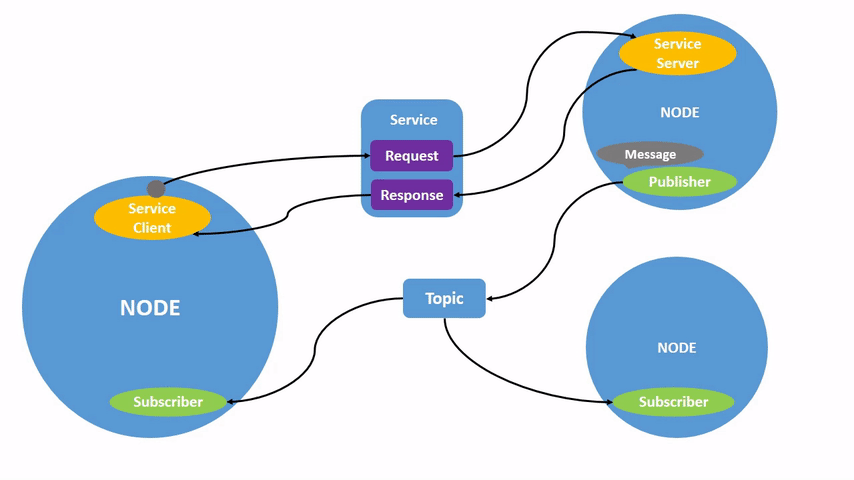
\includegraphics[width=0.8\textwidth,keepaspectratio]{gambar/diagram-node-ros2.png}
  \caption{Diagram komunikasi antar-\emph{node} melalui \emph{topic} dan \emph{service} yang ada pada ROS 2 \citep{url:understandingros2nodes}.}
  \label{fig:diagramnoderos2}
\end{sidewaysfigure}

\begin{sidewaysfigure}
  \centering
  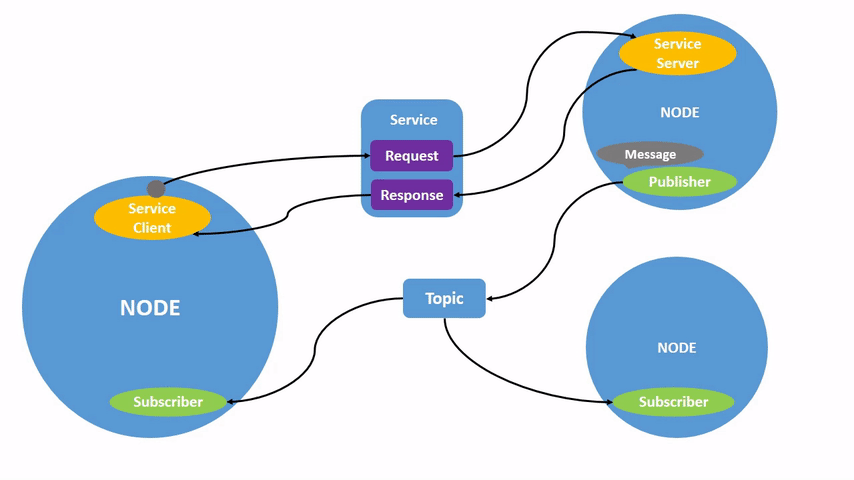
\includegraphics[width=0.8\textwidth,keepaspectratio]{gambar/diagram-action-ros2.png}
  \caption{Diagram komunikasi antar-\emph{node} melalui \emph{action} yang ada pada ROS 2 \citep{url:understandingros2actions}.}
  \label{fig:diagramactionros2}
\end{sidewaysfigure}

Selain \emph{topic} dan \emph{service},
  ROS 2 juga mengenal bentuk lain dari jalur komunikasi antar-\emph{node} yang disebut sebagai \emph{action}.
\emph{Action} merupakan bentuk kompleks dari \emph{topic} dan \emph{service} dimana selain menerima data \emph{response},
  suatu \emph{node} juga dapat menerima data \emph{feedback} secara terus menerus sampai proses yang dijalankan selesai.
Seperti yang terlihat pada Gambar \ref{fig:diagramactionros2},
  suatu \emph{node} dengan \emph{action client} akan mengirimkan data \emph{goal service} melalui sebuah \emph{action} kepada \emph{node} lain dengan \emph{action server} yang terhubung kepada \emph{action} tersebut.
Nantinya, selama proses yang dilakukan oleh \emph{node} dengan \emph{action server} belum selesai,
  \emph{node} tersebut dapat mengirimkan data \emph{feedback topic} kepada \emph{node} dengan \emph{action client}.
Terakhir, jika proses selesai, \emph{node} dengan \emph{action client} dapat mengirimkan data \emph{result service} yang nantinya dapat direspon oleh \emph{node} dengan \emph{action server}.
